\documentclass[border=10pt]{standalone}
\usepackage{times}
\usepackage{tikz}
\usetikzlibrary{positioning, arrows.meta}
\begin{document}
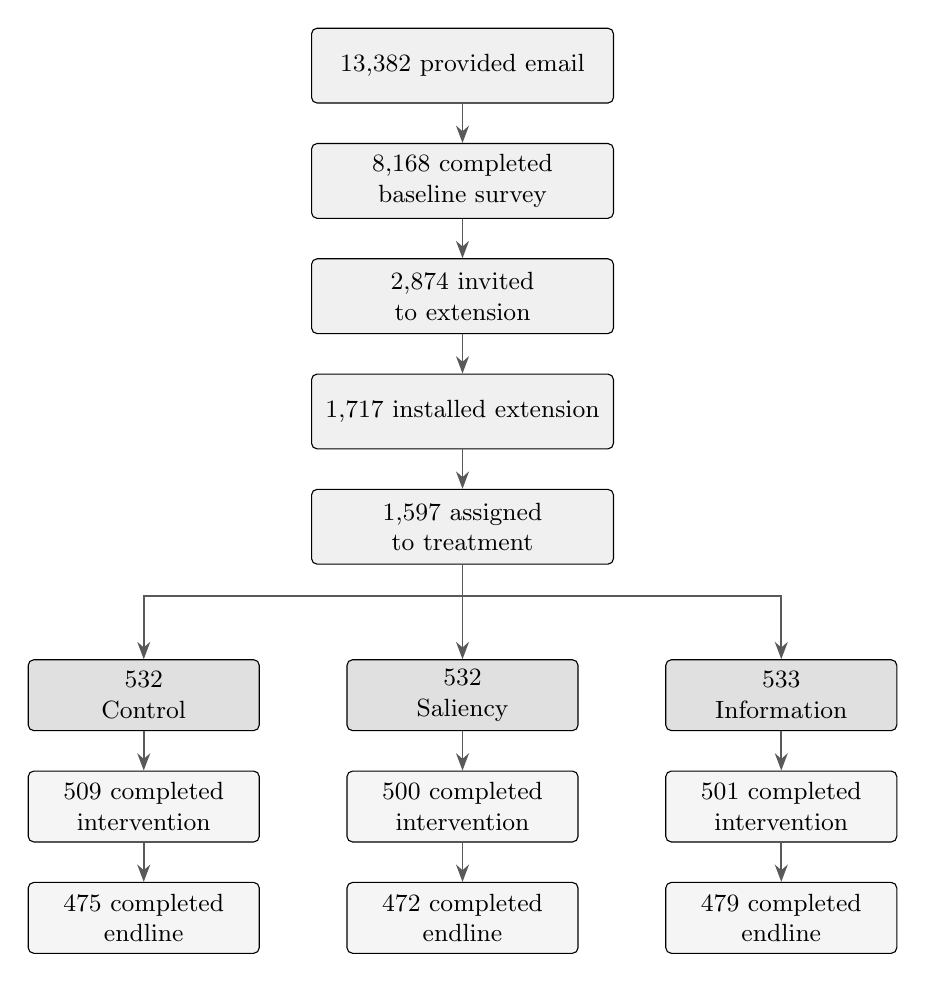
\begin{tikzpicture}[
  font=\small,
  >={Stealth[length=2.2mm]},
  fbox/.style={draw, rounded corners=2pt, align=center, text width=3.6cm,
               minimum height=0.95cm, fill=black!6},
  abox/.style={draw, rounded corners=2pt, align=center, text width=2.7cm,
               minimum height=0.9cm, fill=black!4},
  ahead/.style={draw, rounded corners=2pt, align=center, text width=2.7cm,
                minimum height=0.9cm, fill=black!12},
  arr/.style={->, semithick, draw=black!65},
  node distance=0.5cm,
]
% ---- recruitment funnel ----
\node[fbox] (f1) {13,382 provided email};
\node[fbox, below=of f1] (f2) {8,168 completed baseline survey};
\node[fbox, below=of f2] (f3) {2,874 invited to extension};
\node[fbox, below=of f3] (f4) {1,717 installed extension};
\node[fbox, below=of f4] (f5) {1,597 assigned to treatment};
\draw[arr] (f1)--(f2);
\draw[arr] (f2)--(f3);
\draw[arr] (f3)--(f4);
\draw[arr] (f4)--(f5);
% ---- three arms (Control / Saliency / Information) ----
\node[ahead, below=1.2cm of f5] (sal1)  {532\\Saliency};
\node[ahead, left=1.1cm of sal1] (ctrl1) {532\\Control};
\node[ahead, right=1.1cm of sal1] (info1) {533\\Information};
\node[abox, below=of ctrl1] (ctrl2) {509 completed\\intervention};
\node[abox, below=of sal1]  (sal2)  {500 completed\\intervention};
\node[abox, below=of info1] (info2) {501 completed\\intervention};
\node[abox, below=of ctrl2] (ctrl3) {475 completed\\endline};
\node[abox, below=of sal2]  (sal3)  {472 completed\\endline};
\node[abox, below=of info2] (info3) {479 completed\\endline};
% ---- branch from f5 ----
\draw[arr] (f5.south) -- (sal1.north);
\draw[arr] (f5.south) -- ++(0,-0.4) -| (ctrl1.north);
\draw[arr] (f5.south) -- ++(0,-0.4) -| (info1.north);
% ---- within-arm flow ----
\draw[arr] (ctrl1)--(ctrl2); \draw[arr] (ctrl2)--(ctrl3);
\draw[arr] (sal1)--(sal2);   \draw[arr] (sal2)--(sal3);
\draw[arr] (info1)--(info2); \draw[arr] (info2)--(info3);
\end{tikzpicture}
\end{document}
